
\title{Project Ingenieurswetenschappen: \\ Elektronisch ontwerp van de e-VUBOX \\ Doe-het-zelf bundel}
\author{Vrije Universiteit Brussel}
\date{Versie 08.2015}

\documentclass{exam}
\usepackage[a4paper]{geometry}
\usepackage[T1]{fontenc}
\usepackage[dutch]{babel}
\usepackage{amsmath}
\usepackage{pdflscape}
\newtheorem{DIY}{Doe-het-zelf}
\usepackage{multicol}
\usepackage{enumerate}

%%% FIGURES %%%
\usepackage[pdftex]{graphicx}
\usepackage{caption,subcaption}
\usepackage{hyperref}
\graphicspath{ {./figs/} }

\begin{document}

\maketitle
	\printanswers


	\begin{questions}
\section{Elektronica: componenten en netwerken}

		\question 
			Waarom moeten we een versterker plaatsen tussen het muzieksignaal en de luidspreker?
			\begin{solutionordottedlines}[0.5in]
				Om het vermogen (energie) te versterken van het muzieksignaal, zodat de luidspreker genoeg energie heeft om luid te klinken.
			\end{solutionordottedlines}

		\question 
			Er is tussen twee punten van een netwerk een spanning V:
			\begin{align*}
			    V(t)  = 3~V + 1~V \cdot sin(2\pi \cdot 10~Hz \cdot t)
			\end{align*}
			Welke gedeelte van de spanning is DC, welk gedeelte is AC?
			
			\begin{solutionordottedlines}[0.5in]
				\begin{align*}
					V_{DC} &= 3~V \\
					V_{AC} &= 1~V \cdot sin(2\pi \cdot 10~Hz \cdot t)
				\end{align*} 
			\end{solutionordottedlines}

		\question 
			We hebben een vaste spanning over een weerstand en we willen een grote stroom laten vloeien. Welke weerstand kiezen we dan?
			\begin{choices}
				\choice een grote weerstand (hoge $R$)
				\CorrectChoice een kleine weerstand (kleine $R$)
			\end{choices}

\section{Netwerken}
		
		\question 
			\begin{figure}[h!]
				\centering
				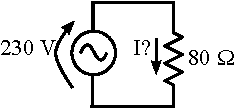
\includegraphics{vbweerstand.pdf}
				\caption{Voorbeeldnetwerkje.}
				\label{fig:vbweerstand}
			\end{figure}
			Een spanningsbron legt een wisselspanning (AC) op met een amplitude van $230~V$ over een weerstand van $80~\Omega$. (Dit is wat er gebeurt in een broodrooster, de weerstand is de gloeidraad die opwarmt en het brood bakt!) Wat is de amplitude van de  stroom $I$ door de weerstand? Wat is het elektrisch vermogen $P$ van de weerstand, die dan in warmte wordt omgevormd?			
			\begin{solutionordottedlines}[1in]
				\begin{align*}
				    I &= V/R \\ &= 230~V/80~\Omega = 2.875 A \\
				    P &= V \cdot I = V^2/R \\ &= (230~V)^2/80~\Omega = 661.25~W \\
				    I&= 2.875~A \hspace{10em}P=  661.25~W 
				\end{align*}

			\end{solutionordottedlines}

		\question
			 Pas de stroomwet van Kirchhoff toe in figuur \ref{subfig:kcl_oef}, en vind de missende stromen. Doe hetzelfde voor de spanningen in figuur \ref{subfig:kvl_oef}.
			\begin{align*}
			    I_S &= \ldots & V_1 = \ldots\\
			    I_R &= \ldots & V_2 = \ldots
			\end{align*}
			\begin{figure}[htbp]
				\centering
				\begin{subfigure}[b]{0.45\linewidth}
					\centering
					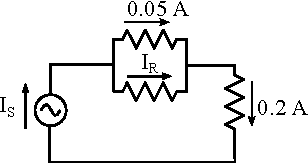
\includegraphics{kcl_oef.pdf}
					\caption{Vind $I_R$ en $I_s$.}
					\label{subfig:kcl_oef}
				\end{subfigure}
				~
				\begin{subfigure}[b]{0.45\linewidth}
					\centering
					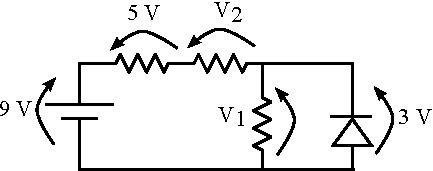
\includegraphics[width=\linewidth]{kvl_oef.pdf}
					\caption{Vind $V_R$ en $U_C$. }
					\label{subfig:kvl_oef}
				\end{subfigure}
			\caption{De wetten van Kirchhoff}
			\label{fig:kirchoff_oef}
			\end{figure}

			\begin{solutionordottedlines}[2in]
				\begin{align*}
					\intertext{Stroomwetten:}
					&I_S = 0.05A + I_R \\
					&I_R + 0.05A = 0.2A \\
					&I_S = 0.2A
					\intertext{Oplossing:}
					&I_R = 0.2A - 0.05A = 0.15A \\
					&I_S = 0.2 A
				\end{align*}

				\begin{align*}
					\intertext{Spanningswetten:}
					&V_1-3V = 0 \\
					&9V-5V-V_2-V_1 = 0 \\
					\intertext{Oplossing:}
					&V_1 = 3V \\
					&V_2 = 9V-5V-3V = 1V
				\end{align*}

				\begin{align*}
					I_S &= 0.20~A & V_1 = 3~V\\
					I_R &= 0.05~A  & V_2 =1~V 
				\end{align*}
			\end{solutionordottedlines}

\section{Bouwstenen van de e-VUBOX}
\subsection{De volumeknop: de weerstandsdeler}
		\question
			\begin{figure}[htbp]
				\centering
				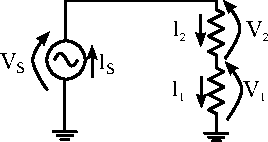
\includegraphics{weerstandsdeler}
				\caption{Volumeregeling: de spanningsdeler}
				\label{fig:volume}
			\end{figure}
			Je hebt een voltage van $9$ V als ingangsspanning $V_S$, en je wilt een voltage van $1.5$ V als uitgangsspanning $V_2$. $R_1$ is al gekozen en heeft een weerstand van $1$ k$\Omega$ ($1000 \Omega$). Welke waarde moet je kiezen voor $R_2$?
				\begin{align*}
				    R_2 = \ldots\ldots
				\end{align*}
				Let op! Bestaat die weerstandswaarde wel? Kies een bestaande waarde uit de E12-reeks.

			\begin{solutionordottedlines}[1in]
					\begin{align}
					    \frac{R_1}{R_1+R_2} &= \frac{1.5V}{9V} \\
					    \frac{1 k\Omega}{1k\Omega + R_2} &= \frac{1}{6}\\
					    \frac{1k\Omega + R_2}{1 k\Omega} &= 6\\
					    1k\Omega + R_2 &= 6 \cdot 1k\Omega\\
					    R_2 &= 6 \cdot 1 k\Omega - 1 k\Omega =  5 k\Omega  \\
					    \intertext{maar deze waarde is geen E12-waarde, we kiezen dus:}
					    R_2 &= 4.7 k\Omega
					\end{align}
			\end{solutionordottedlines}

		\question
			 Welke weerstand $R_{pot}$ moet de potentiometer hebben, wetend dat de ingangsspanning $V$ maximaal $200$ mV ( = $200 \cdot 10^{-3}$ V) is en we het vermogen $P$ door de potentiometer willen beperken tot 4 $\mu$W ( = $4 \cdot 10^{-6}$ W)? 
			\begin{align*}
			    R_{pot} = \ldots\ldots
			\end{align*}

			\begin{solutionordottedlines}[1in]
				\begin{align*}
					P &= V \cdot I = V^2 / R_{pot} \\
					R_{pot} &= (200mW)/4\mu W \\
				    R_{pot} &= 10 k\Omega
				\end{align*}
			\end{solutionordottedlines}

\subsection{Het statusledje: de diode}
		\question
			\begin{figure}[htbp]
				\centering
				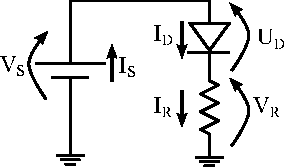
\includegraphics{diode_netwerk}
				\caption{Diode netwerk.}
				\label{fig:diode_netwerk}
			\end{figure}

			De spanningsbron die we gaan gebruiken voor onze versterker is een 9V batterij, dus $V_s = 9$ V. We zijn op zoek naar de weerstand die nodig is zodat $U_D = 1.8$ V en $I_D =10$ mA. Gebruik de wetten van Kirchhoff in het netwerk \ref{fig:diode_netwerk}:
				\begin{align}
					+V_s &- U_D - V_R = 0  \\
					I_s &= I_D = I_R
				\end{align}
				 Kan je de waarde vinden van de weerstand die nodig is? \textbf{Tip:} bepaal $I_R$ en $V_R$ uit de wetten van Kirchhoff.
				\begin{align*}
				    R_{led} = \ldots\ldots
				\end{align*}

			\begin{solutionordottedlines}[1in]
				\begin{align*}
					\intertext{Kirchhoff:}
						V_S &- U_D - V_R = 0 \\
						I_S &= I_D = I_R \\
					\intertext{De weerstand die nodig is:}	
					    R_{led} &= \frac{V_R}{I_R} \\
					    		&= \frac{V_S-U_D}{I_D} \\
					    		&= \frac{9V-1.8V}{10mA} \\
					    		&= \frac{7.2V}{10mA} = 720 \Omega \\
					\intertext{We kiezen een weerstand in de E12 reeks:}
					    R_{led} &= 680 \Omega
				\end{align*}
			\end{solutionordottedlines}

\subsection{De versterker: de transistor}
		\question
			\begin{align}
					    I_C = -\frac{\beta}{\beta+1}I_E
			\end{align}
			Elimineer $\beta$ van de vorige vergelijking door de volgende limiet op te lossen.

			\begin{align*}
			    I_C \approx \lim_{\beta \rightarrow \infty} -\frac{\beta}{\beta+1}I_E = \ldots
			\end{align*}
			
			\begin{solutionordottedlines}[1in]

				\begin{align*}
					I_C \approx \lim_{\beta \rightarrow \infty} -\frac{\beta}{\beta+1}I_E = \lim_{\beta \rightarrow \infty} -\frac{\beta}{\beta}I_E = -I_E
				\end{align*}
			
			\end{solutionordottedlines}


		\question
			\begin{figure}[htbp]
				\centering
				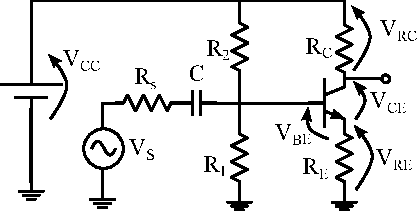
\includegraphics{ges}
				\caption{Versterkerschakeling met de transistor.}
				\label{fig:ges}
			\end{figure}
			\begin{align}
				V_C &= V_{CC} - V_{R_C} = V_{CC} - \frac{R_C}{R_E} \cdot (V_B - 0.7~V)
				\label{eq:versterking}
			\end{align}		

			Door de ontkoppelcapaciteit $C$ en de weerstandsdeler $R_1R_2$ is
			
			\begin{align*}
			    V_B = \frac{R_1}{R_1+R_2}V_{CC} +V_S
			\end{align*}

			 $V_{CC}$ is een DC spanning, de muziek $V_S$ is een AC spanning. Vul dit in vergelijking \ref{eq:versterking}, en  splits de spanning $V_C$ op in een AC en DC gedeelte:
			\begin{align*}
			    (AC)~v_C = \ldots \\ (DC)~V_C = \ldots & 
			\end{align*}

			\begin{solutionordottedlines}[1in]
					\begin{align*}
					V_C &= V_{CC} - V_{R_C} = V_{CC} - \frac{R_C}{R_E} \cdot (\frac{R_1}{R_1+R_2}V_{CC} +V_S - 0.7~V) \\
					V_{DC} &= V_{CC} - \frac{R_C}{R_E} \cdot (\frac{R_1}{R_1+R_2}V_{CC} - 0.7~V) \\
					V_{AC} &= - \frac{R_C}{R_E} \cdot V_S
				\end{align*} 
			\end{solutionordottedlines}

		\question
		We hebben gekozen:
			\begin{align}
				I_C = 10~mA \\
			    V_C =  3.5~V \\
			    -\frac{R_C}{R_E} = -5
			\end{align}

			Je kent nu alles wat nodig is om de weerstanden $R_{E}$ en $ R_{C}$ te bepalen. \textbf{Tip:} $V_{R_C} = V_CC - V_C$
				\begin{align}
				    R_C &= \ldots \\
				    R_E &= \ldots
				\end{align}

			\begin{solutionordottedlines}[1in]
					\begin{align}
						R_C &= \frac{ V_{R_C}}{I_{R_C}} = \frac{V_{CC}-V_C}{I_C}= \frac{9V - 3.5V}{10mA} = 550 \Omega \\
						R_E &= \frac{R_C}{5} = 110 \Omega 
						\intertext{Weerstanden in E12 series:}
						R_C &= 560 \Omega\\
						R_E &= 100 \Omega
					\end{align}
			\end{solutionordottedlines}

		\question
			Bereken het biasvoltage $V_B$ uit $V_E$. Kies dan de weerstand $R_2$ zodat de uitgangspanning $V_B$ de gewenste waarde heeft. Het staat al vast dat $R_1 = 1k\Omega$. \textbf{Tip:} Vergeet niet de ingansspanning $V_{CC}$ is $9V$.

			\begin{align}
				V_B &= \ldots \\
			    R_1 &= 1k\Omega \\
			    R_2 &= \ldots
			\end{align}

			\begin{solutionordottedlines}[1in]
				\begin{align*}
					\intertext{Biasvoltage:}
					    V_B &= V_E + 0.7V = R_E \cdot (-I_E) = 100 \Omega \cdot 10 mA  + 0.7V = 1.7V
					\intertext{Weerstandsdeler:}
					    V_B &= \frac{R_1}{R_1+R_2}V_{CC} \\
					    \frac{V_B}{V_{CC}} &= \frac{R_1}{R_1+R_2} \\
					    \frac{V_{CC}}{V_B} &= \frac{R_1+R_2}{R_1} \\
					    \frac{V_{CC}}{V_B} \cdot R_1 - R_1 &= R_2 \\
					    \frac{9V}{1.7V} \cdot 1k\Omega - 1k\Omega &= R_2 \\
					    R_2 &= 5.29 \cdot 1k\Omega -  1k\Omega \\
					    R_2 &= 4.29 k\Omega\\
					    \intertext{Weerstand in de E12-serie, een beetje groter genomen om stroom te beperken}
					    R_2 &= 4.8 k\Omega
					\end{align*}
			\end{solutionordottedlines}	

\subsection{De luidspreker: de (slechte) weerstand}

		\question
			Bereken het gemiddeld vermogen via de integraal:
			\begin{align*}
			   P_{gemm} = \frac{1}{1/440 \text{Hz}} \int_0^{1/440Hz} 1.125~\text{W} \cdot \sin^2 \left(2\pi \cdot 440~\text{Hz} \cdot t\right) dt
			\end{align*}

			Met behulp van de goniometrische formule:
			\begin{align*}
			    \sin^2(\theta) = \frac{1 - \cos(2\theta)}{2}
			\end{align*}

		 	\begin{align*}
			    P_{gemm} = \ldots
			\end{align*}

			\begin{solutionordottedlines}[3in]
			\begin{align*}
			    P_{gemm} 	&= \frac{1}{1/440 \text{Hz}} \int_0^{1/440Hz} 1.125~\text{W} \cdot \sin^2 \left(2\pi \cdot 440~\text{Hz} \cdot t\right) dt \\
			    			&=\frac{1.125~\text{W}}{2 \cdot 1/440 \text{Hz}} \int_0^{1/440Hz} (1- \cos(4\pi \cdot 440~\text{Hz} \cdot t) dt \\
			    			&=\frac{1.125~\text{W}}{2 \cdot 1/440 \text{Hz}} \int_0^{1/440Hz} 1 \cdot dt - \int_0^{1/440Hz} \cos(4\pi \cdot 440~\text{Hz} \cdot t) dt \\
			    			&=\frac{1.125~\text{W}}{2 \cdot 1/440 \text{Hz}} t\bigg|^{1/440 \text{Hz}}_0 - 0 \\
			    			&= \frac{1.125~\text{W}}{2 \cdot 1/440 \text{Hz}} (1/440 \text{Hz} - 0)\\
			    			&= \frac{{1.125~\text{W}}}{2}\\
			    			&\approx 560~mW
			\end{align*}

			\end{solutionordottedlines}	
	\end{questions}

\end{document}
